\documentclass{article}
\usepackage[utf8]{inputenc}
% 15, 22, 20 et 20
\usepackage[top = 5 mm, bottom = 5 mm, left = 8 mm, right = 8 mm]{geometry}
\usepackage{rotating, graphicx}
\usepackage{blindtext, rotating}
\usepackage[english]{babel}
\usepackage{amsmath}
\usepackage{graphicx}
\usepackage{subcaption}
\usepackage[colorinlistoftodos]{todonotes}
\usepackage{rotfloat}
\usepackage[utf8]{inputenc}
\usepackage[T1]{fontenc}
\usepackage{amssymb}
\usepackage{color}
\usepackage{fancyhdr}
\usepackage{xcolor}
\usepackage{tikz}
\usepackage{caption}
\usepackage{enumerate}
\usepackage{pgfplots}
\usepackage{caption}
\usepackage{hyperref}
\usepackage{circuitikz}
\usepackage{newfloat}
\usepackage{float}
\usepackage{array}
\usepackage{eurosym}
\usepackage{multirow}
\usepackage{enumitem}
\usepackage[version=3]{mhchem}
\usepackage{amssymb}
\usepackage{schemata}
\usepackage{tcolorbox}
\usepackage{algorithm}
\usepackage{algorithmic}
\usepackage[nottoc]{tocbibind}
\usepackage{mathtools}
\usepackage{booktabs} 

\usepackage{listings}
\lstset{language=Python}
\pgfplotsset{compat=1.15} 

\DeclareUnicodeCharacter{20AC}{\euro{}}
\definecolor{UCLblue}{RGB}{14,43,88}

\newcommand{\HRule}{\rule{\linewidth}{0.5mm}}
\newcommand*{\QEDB}{\hfill\ensuremath{\square}}%
\newcommand\SB[2]{\schema{\schemabox{\textbf{#1}}}{\schemabox{#2}}}


\begin{document}

\begin{titlepage}
    \fontfamily{qag}\selectfont
    \color{UCLblue}
    \bfseries
    \begin{center}

    \begin{figure}
        \centering
        \includegraphics[width=0.6\linewidth]{Images/UCLouvain_Logo.eps}
    \end{figure}

    {\LARGE École Polytechnique de Louvain}\\[1cm]

    {\Large LEPL1110 - Eléments finis}\\[1.5cm]
    % Title
    \HRule \\[0.4cm]
    { \huge \bfseries Projet : Problème d'élasticité linéaire \\[0.2cm] }
    \HRule \\[1cm]
    \huge{\today}
    \vfill
    \large
      \begin{tabular}{l}
            
        Mathis \textsc{Delsart} - 31302100\\
        Adrien \textsc{Antonutti} - 31202100\\
        \\
        Gatien \textsc{Dony} - Tuteur de référence\\
        Simon \textsc{Yans} - Assistant de référence\\
        
      \end{tabular}
        ~\\
    \vfill
      \begin{center} \large
        \emph{}\\
        
        \hspace{40pt}
        \end{center}
    {\large 2023 - 2024}
  \end{center}
\end{titlepage}
\newpage

\newpage
%%%%%%%%%%%%%%%%%%%%%%%%%%%%%%%%%%
%%%%%%%%%%%%%%%%%%%%%%%%%%%%%%%%%%
\setlength{\parindent}{0cm}

\section{Introduction}

Les ponts représentent des éléments cruciaux de l'infrastructure urbaine, assurant la connectivité et la mobilité. Notre étude se concentre sur la modélisation et l'analyse d'un pont, une structure essentielle pour le déplacement des personnes et des véhicules. La particularité de notre projet réside dans la présence d'un tunnel piétonnier/cycliste associé, incitant les individus à choisir des modes de déplacement écologiques. Cette transition soutient notre engagement en faveur de la durabilité et de la réduction des émissions de carbone dans les zones urbaines.

\section{Description géométrique du problème}
\label{geometry}

Notre géométrie, illustrée à la figure \ref{fig:geometry}, est un pont soutenu par quatre piliers, comportant deux colonnes principales qui supportent des câbles à la manière des ponts à haubans, assurant ainsi la stabilité de la structure. Des arches de tailles variables sont également présentes. De plus, un tunnel piétonnier/cycliste est aménagé sous les arches, doté de fenêtres sur les côtés.

\begin{figure}[H]
    \centering
    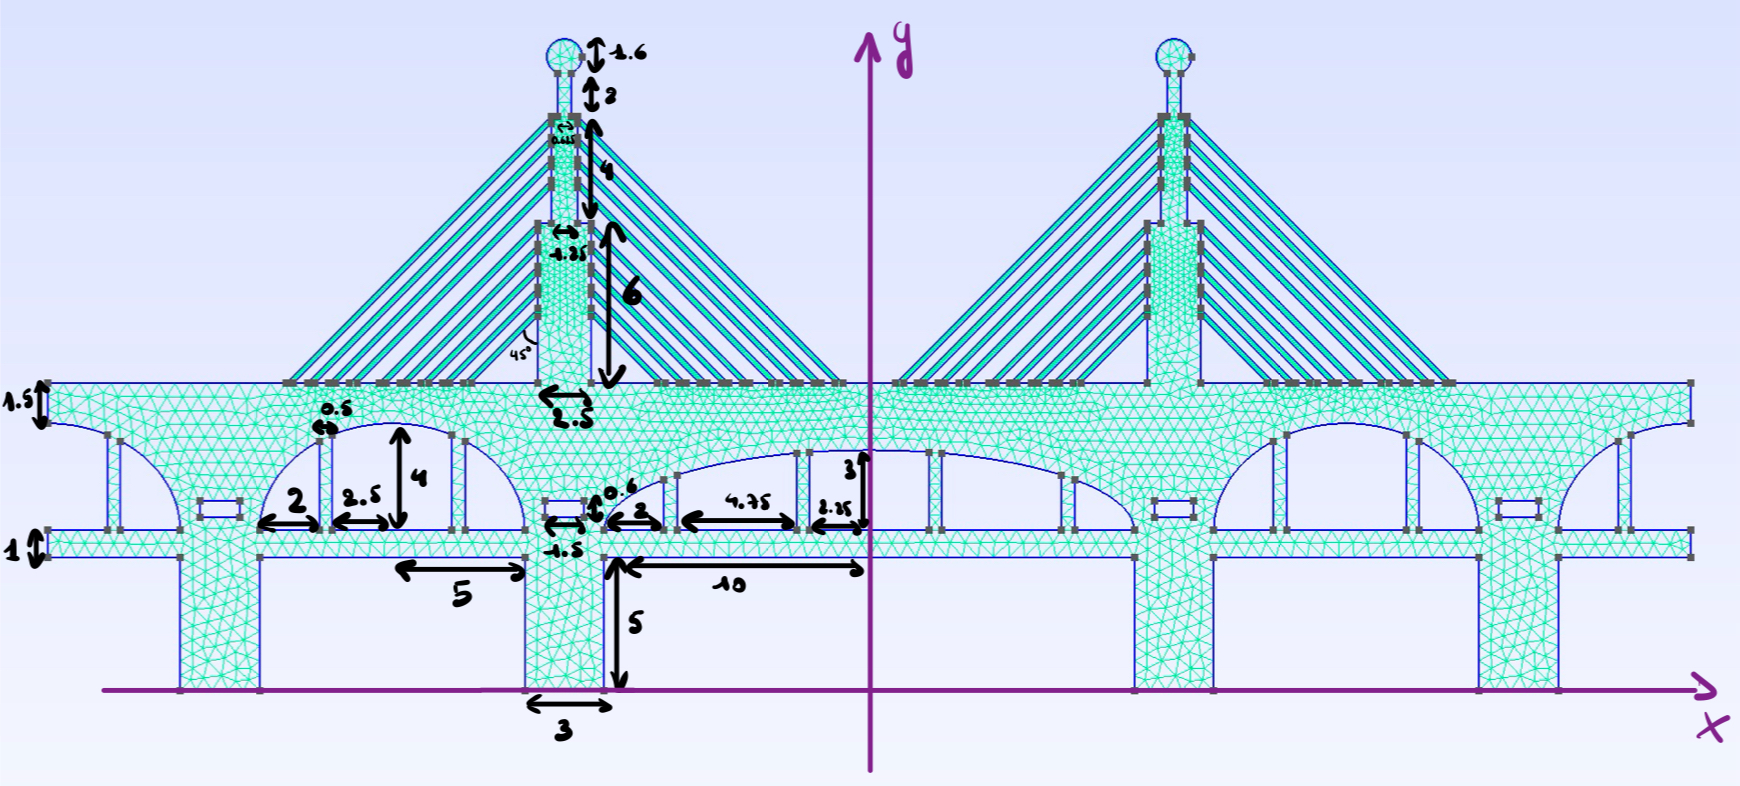
\includegraphics[width=12cm]{Images/GeometryProblem.png}
    \caption{Géométrie du problème}
    \label{fig:geometry}
\end{figure}

Notre géométrie possède une symétrie par rapport à l'axe des ordonnées, ce qui réduit la complexité du modèle. Seules les dimensions essentielles ont été explicitement notées, tandis que les autres peuvent être déduites de manière aisée grâce à cette symétrie. Cette caractéristique symétrique nous permettra, lors des simulations, de ne considérer que la partie gauche de la géométrie, c'est-à-dire : $\forall (x,y) \in \text{Domaine}, \quad x \leq 0$.


\section{Maillage caractéristique de la géométrie}
\label{"mesh"}

Le maillage caractéristique de notre géométrie presentée à la section \ref{geometry}, généré avec gmsh, est illustré à la figure \ref{fig:mesh_gmsh}.

Nous avons uniquement maillé la partie gauche de notre géométrie car nous ne simulerons que celle-ci par symétrie. Celui-ci a été réalisé par des interpolations d'hermite sur les frontières et les endroits qui nous semblait pertinent à observer lors des simulations comme par exemple les câbles, les colonnes et évidemment les tabliers du pont.

Nous disposons également de fonctions permettant de déterminer si un point $(x, y)$ appartient à un des tabliers ou un des câbles dans la géométrie. Cela nous permettra d'adapter le matériau et la taille du maillage en fonction de ces positions, assurant ainsi une modélisation précise des zones sensibles de la structure. Une analyse plus approfondie sur les matériaux utilisé est présentée dans la section \ref{"materials"}.

\begin{figure}[H]
     \centering
     \hspace{0cm}
     \begin{subfigure}[b]{0.6\textwidth}
         \centering
         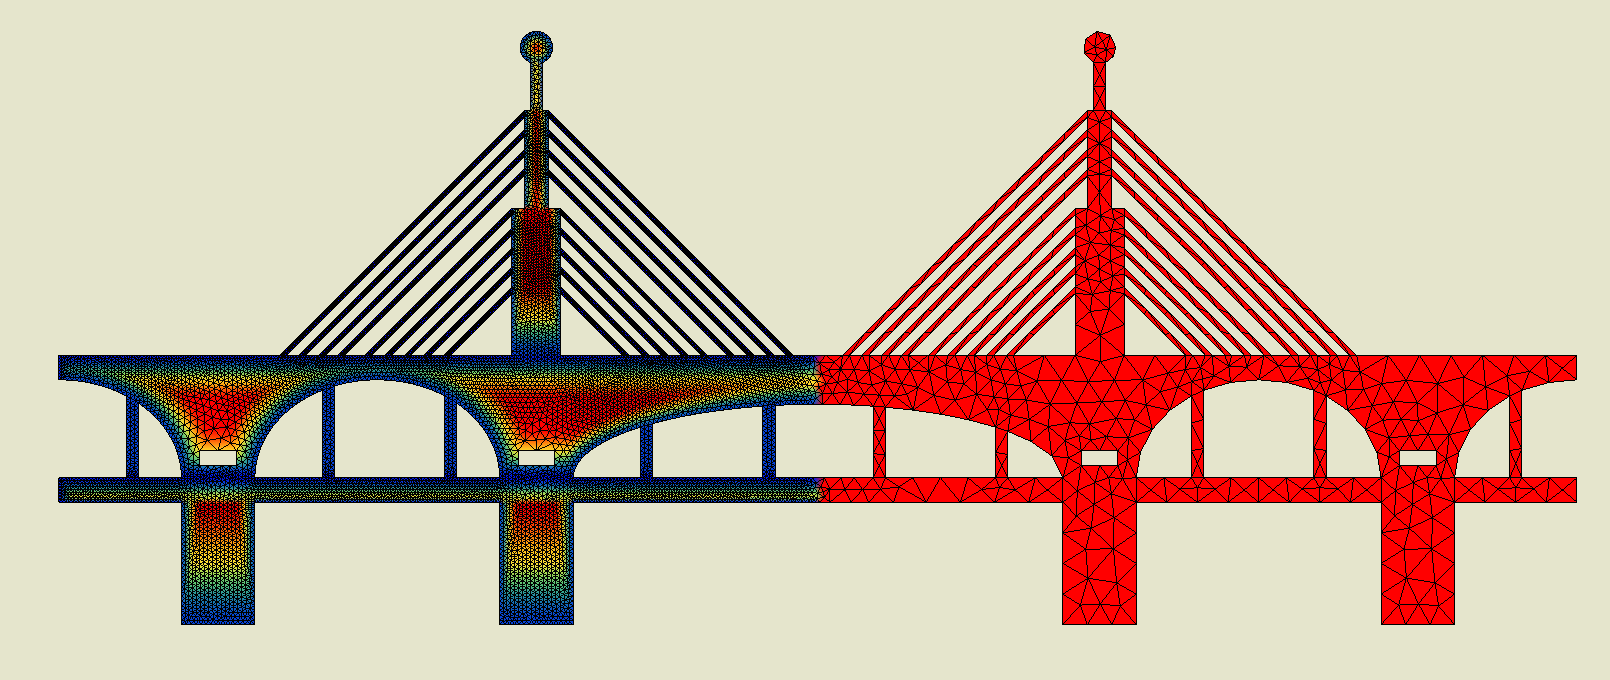
\includegraphics[width=\textwidth]{Images/geometry.png}
         \caption{Maillage complet}
         \label{fig:meshAll}
     \end{subfigure}
     \hspace{0cm}
     \begin{subfigure}[b]{0.3\textwidth}
         \centering
         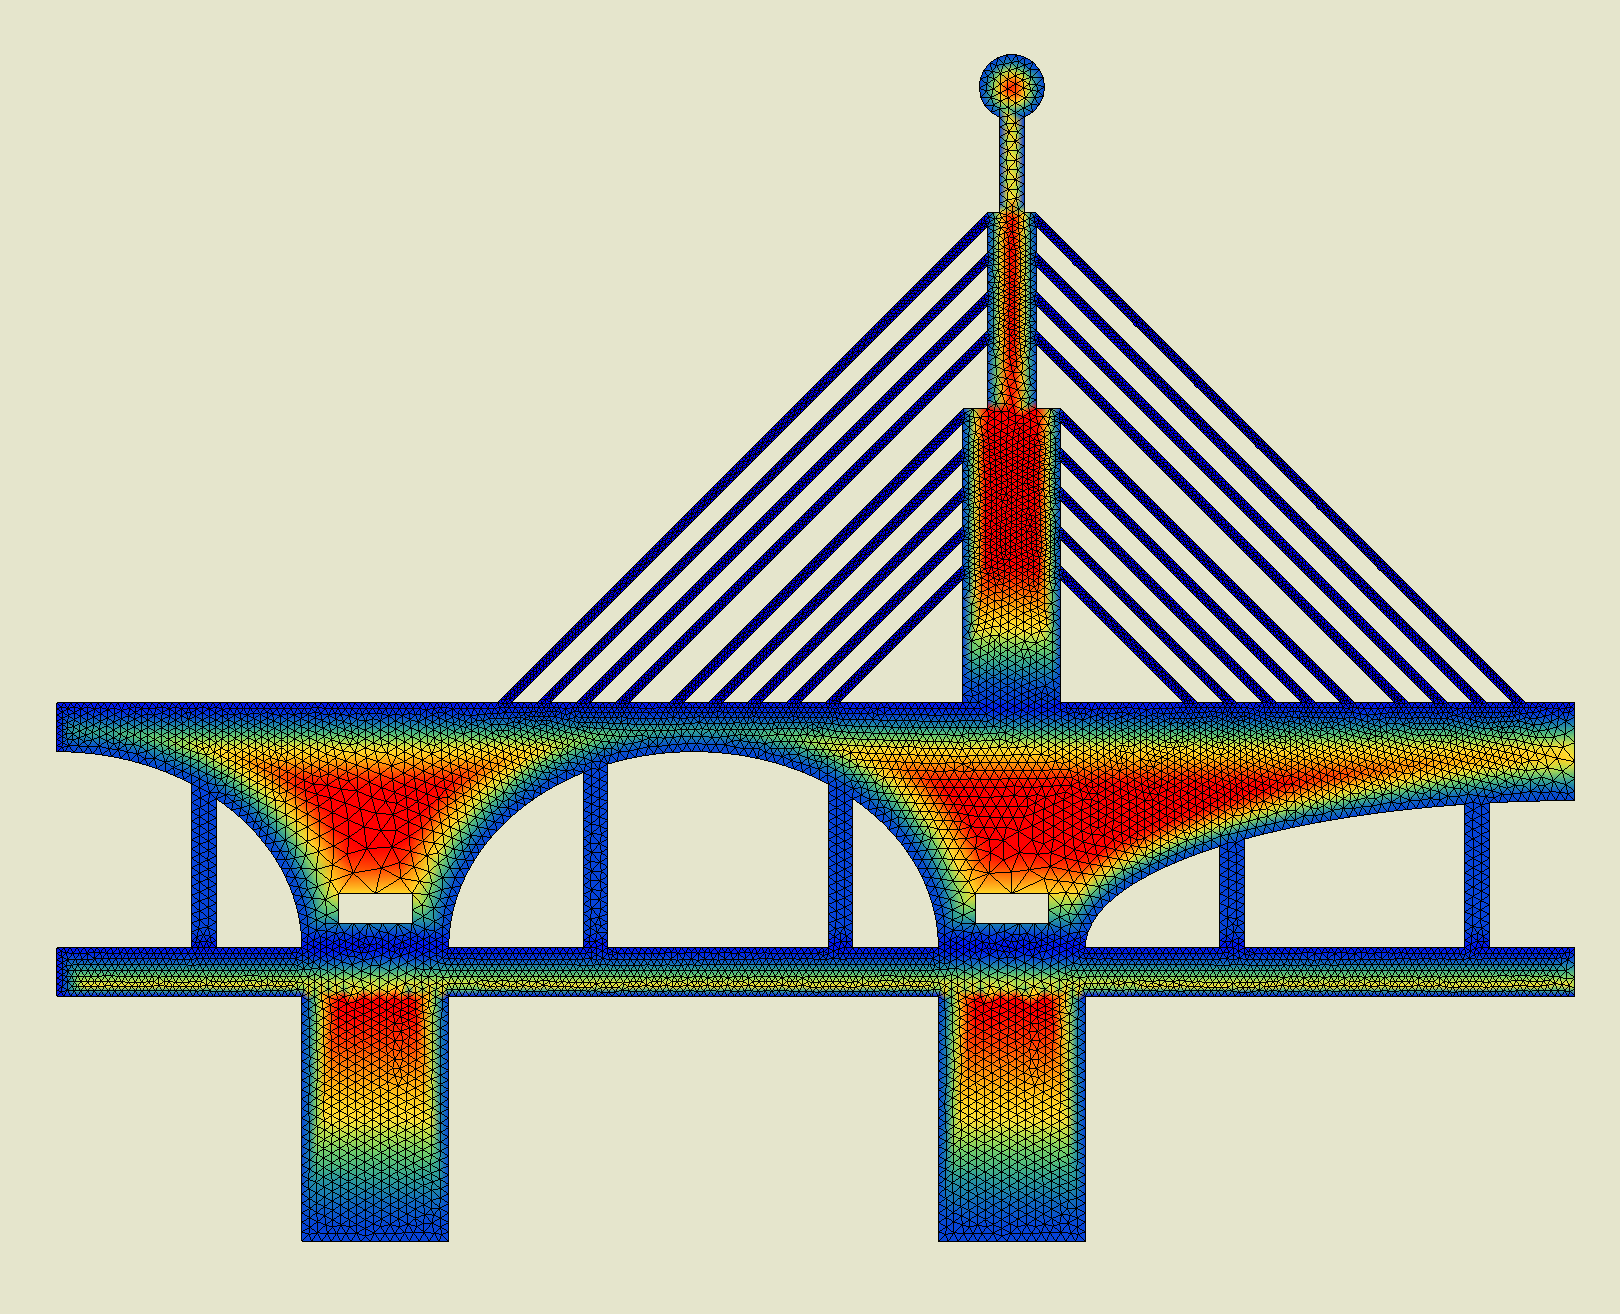
\includegraphics[width=\textwidth]{Images/mesh_geometry.png}
         \caption{Partie gauche symétrique du maillage}
         \label{fig:meshLeft}
     \end{subfigure}
     
        \caption{Maillage caractéristique de notre géométrie généré avec gmsh}
        \label{fig:mesh_gmsh}
\end{figure}


\section{Description des conditions aux frontières}

Nous allons utiliser l'hypothèse de tension plane pour généraliser la loi de Hooke 3D à notre problème 2D, étant donné que notre pont peut se déformer sur les côtés. Cela engendre des contraintes nulles dans la direction perpendiculaire au plan (x, y).

Pour les conditions aux frontières, nous commençons par imposer un déplacement nul selon les axes x et y sur les trois frontières des quatre gros piliers ainsi que sur les deux parois latérales du pont. Ces conditions de déplacement nul permettent de fixer le pont en empêchant tout mouvement du corps rigide.
Ensuite, nous imposons une contrainte le long de l'axe x, correspondant à la force appliquée par le vent sur la surface modélisant l'effet du vent sur la structure.
Nous imposerons aussi des forces variables exercées sur les tabliers en fonction des charges appliquées, ainsi qu'un déplacement libre.
Pour finir, nous appliquons une condition de symétrie sur l'axe des y, car il s'agit de l'axe de symétrie de la structure (cfr. \ref{fig:geometry}). Cette approche réduira le temps de calcul des simulations car nous prendrons en compte uniquement la moitié de la géométrie pour le maillage (cfr. \ref{fig:meshLeft}). Nous ne perdrons aucune solution pour l'ensemble de la géométrie car les déplacements et les contraintes sont symétriques de part et d'autre de l'axe de symétrie. De plus, la condition frontière que nous appliquerons aux points de rupture du pont est celle d'un déplacement nul selon l'axe x. Cela s'explique par le fait que lorsque le pont n'est pas rompu, les forces internes s'annulent mutuellement, ce qui entraîne un déplacement nul dans la direction x.

\section{Paramètres des matériaux}
\label{"materials"}
Pour assurer la robustesse de notre structure, nous avons sélectionné des matériaux spécifiques en fonction de leurs caractéristiques. Nous utilisons de l'acier pour les câbles et les tabliers, car il résiste bien à la traction. En revanche, le béton armé est utilisé pour le reste de la structure en raison de sa capacité à résister à la compression. Comme abordé dans la section \ref{"mesh"}, nous avons mis en place des fonctions qui permettent, pour chaque triangle du maillage, de récupérer les propriétés du matériau en fonction des coordonnées du centre de gravité du triangle. Cette approche garantit une simulation aussi réaliste que possible. \\

Les paramètres pris en compte pour chaque matériau sont les suivants :
\begin{itemize}
    \item La \textbf{masse volumique} $\rho$ [kg/$m^3$] $\coloneqq$ masse du matériau par unité de volume.
    \item Le \textbf{module de Young} E [N/$m^2$] $\coloneqq$ capacité du matériau à se déformer sous contrainte.
    \item Le \textbf{coefficient de Poisson} $\nu$ [/] $\coloneqq$ relation entre la déformation longitudinale et transversale du matériau sous contrainte.
    \item La \textbf{limite d'élasticité} $R_e$ ou $\sigma_e$ [N/$mm^2$] $\coloneqq$ tension jusqu'à laquelle le matériau peut être déformé de manière élastique (déformation non permanente).
    \item La \textbf{limite à la rupture} $R_r$ ou $\sigma_r$ [N/$mm^2$] $\coloneqq$ contrainte maximale à laquelle un matériau peut être soumis avant de subir une rupture. \\
\end{itemize}

Après avoir effectué quelques recherches, nous avons recueilli les données suivantes :
\begin{table}[htbp]
    \centering
    \caption{Propriétés des matériaux}
    \begin{tabular}{l|ccccc}
        \toprule
        Matériau & $E$ [GPa] & $\nu$ [/] & $\rho$ [kg/m\textsuperscript{3}] & $R_e$ [MPa] & $R_r$ [MPa] \\
        \midrule
        Acier & 200 & 0.3 & 7850 & 380 & 475 \\
        Béton armé & 35 & 0.2 & 2500 & 28 & 35\\
        \bottomrule
    \end{tabular}
    \label{tab:proprietes_materiaux}
\end{table}

\section{Objectifs de simulation}

\begin{itemize}
    \item Déterminer les contraintes dans le pont et identifier les zones critiques en termes de contrainte.
    \item Calculer la charge maximale admissible par le pont avant sa défaillance.
    \item Calculer la flèche maximale au centre du pont sous charge nominale.
    \item Modéliser et simuler les charges variables pour évaluer les effets du trafic routier sur la structure.
    \item Calculer la vitesse théorique maximale du vent entraînant une défaillance du pont.
    \item Analyser les résultats de simulation pour optimiser la géométrie du pont en termes de résistance et de déformations minimales.
    \item \textit{\textbf{Extra}}: Déterminer la fréquence de résonance du pont susceptible de causer des dommages structurels.
    \item \textit{\textbf{Extra}}: Évaluer les effets des vibrations induites par le trafic sur la stabilité du pont.
    \item \textit{\textbf{Extra}}: Examiner les variations de température et leur impact sur les déformations et la stabilité du pont.

\end{itemize}

\end{document}